\documentclass[11pt]{article}
\usepackage[scaled=0.92]{helvet}
\usepackage{geometry}
\geometry{letterpaper,tmargin=1in,bmargin=1in,lmargin=1in,rmargin=1in}
\usepackage[parfill]{parskip} % Activate to begin paragraphs with an empty line rather than an indent %\usepackage{graphicx}
\usepackage{amsmath,amssymb, mathrsfs, dsfont}
\usepackage{mathtools}

\usepackage{tabularx}
\usepackage[font=footnotesize,labelfont=bf]{caption}
\usepackage{graphicx}
\usepackage{xcolor}
%\usepackage[linkbordercolor ={1 1 1} ]{hyperref}
%\usepackage[sf]{titlesec}
\usepackage{natbib}
\usepackage{../../Tianpei_Report}

%\usepackage{appendix}
%\usepackage{algorithm}
%\usepackage{algorithmic}

%\renewcommand{\algorithmicrequire}{\textbf{Input:}}
%\renewcommand{\algorithmicensure}{\textbf{Output:}}



\begin{document}
\title{Lecture 5: Monte Carlo Methods}
\author{Tianpei Xie}
\date{ Aug 4th., 2022 }
\maketitle
\tableofcontents
\newpage
\section{Monte Carlo Methods}
Unlike the previous chapter, here we do not assume complete knowledge of the environment. Since we do not know the precise dynamic function $p$, we cannot use DP to find optimal value and optimal policies. Instead, we can estimate  value functions and discover optimal policies via \emph{sampling}.  \textbf{Monte Carlo methods} require only \emph{experience} -- sample sequences of states, actions, and rewards from actual or simulated interaction with an environment. It either learns from \emph{actual} experience when \emph{no prior knowledge} of the environment’s dynamics is known or learns from \emph{simulated} experiences, when we have model that generate sample transition but not complete as dynamic. 

Monte Carlo Methods are ways of solving the reinforcement learning problem based on \textbf{averaging sample returns}. To ensure that well-defined returns are available, here we define Monte Carlo methods only for \textbf{episodic tasks}. Only \emph{on the \textbf{completion} of an episode} are value estimates and policies changed. Monte Carlo methods can thus be incremental in an \emph{\textbf{episode-by-episode sense}}, but not in a step-by-step (\emph{online}) sense.

Compare to the Bandit problem where we simply sample and average rewards, in Monte Carlo, we sample and \emph{average returns} for each state-action pair. Also the Monte Carlo methods learn value and policy from experience in the form of \emph{sample episodes}.

There are three \textbf{advantages} of using Monte Carlo Methods over DP:
\begin{itemize}
\item \textbf{No need to have complete knowledge on dynamics}:  In DP, all of the probabilities $p(s', r|s, a)$ for all $s', r, s, a$ must be computed before DP can be applied, and such computations are often complex and error-prone. In constrasts, Monte Carlo methods have ability to learn optimal behavior directly from interaction with the environment. It only need sample episodes. 

\item \textbf{They can be used with simulation or \emph{sample models}, which has low expense for computation}: Generating the sample games required by Monte Carlo methods is easy. An important fact about Monte Carlo methods is that the estimates for each state are \textbf{\emph{independent}}. \emph{The estimate for \underline{one state} does not build upon the estimate of \underline{any other state}}, as is the case in DP. In other words, Monte Carlo methods do not \emph{\textbf{\underline{bootstrap}}} as we defined it in the previous chapter.  

\item \textbf{It is easy and efficient to focus Monte Carlo methods on a small subset of the states.}: In particular, note that the computational expense of estimating the value of a single state is \emph{\underline{independent} of the number of states}. This can make Monte Carlo methods particularly attractive when \emph{one requires the value of only one or a subset of states}. One can generate many sample episodes \textbf{starting from the states of interest}, averaging returns from \emph{only these states}, \emph{ignoring} all others. 

\item \textbf{They do not bootstrap} thus it can be used when \textbf{Markov property not hold}. That is they do not update their value estimates on the basis of the value estimates of successor states. They may be less harmed by violations of the Markov property. 
\end{itemize}

Maintaining \emph{\textbf{sufficient exploration}} is an issue in Monte Carlo control methods. It is not enough just to select the actions currently estimated to be best, because then no returns will be obtained for alternative actions, and it may never be learned that they are actually better. 

\section{Monte Carlo Methods for Prediction}
We begin by considering Monte Carlo methods for learning the \emph{state-value function} for a given policy. Note that by definition, the state-value function $v$ 
\begin{align*}
v_{\pi}(s) &= \E{\pi}{G_{t} | S_{t} = s} \\
&\approx \frac{\sum_{t}^{T(s)} G_{t}}{N(s)}\, 
\end{align*} where $N(s) = |T(s)|$ and $T(s) = \{S_{t}=s\}_{t=1}^{\infty}$ or the number of epsiodes for first-visit MC.

Each occurrence of state $s$ in an episode is called a \emph{visit} to $s$. Of course, $s$ may be visited multiple times in the same episode; let us call the first time it is visited in an episode the \emph{first visit} to $s$. The \emph{\textbf{first-visit MC method}} estimates $v_{\pi}(s)$ as the average of the returns \emph{following first visits} to $s$, whereas the \emph{\textbf{every-visit MC method}} averages the returns following \emph{all visits} to $s$. First-visit MC is shown in procedural form in the Figure \ref{fig: First_visit_MC_pred}. Since the \underline{first visit in each epsiodes} are generated \emph{i.i.d}.,  the first-visit MC is easier to analyze, whereas the \underline{every-visit MC} is harder since the within-episode visits are \underline{not independent}.  Every-visit MC would be the same except without the check for $S_t$ having occurred earlier in the episode. Note that the estimation goes \emph{backwards} starting from the end of episode. This way we can apply resursive equation $G_{t} = R_{t+1}+ \gamma\,G_{t+1}$. 

\begin{figure}
\begin{minipage}[t]{1\linewidth}
  \centering
  \centerline{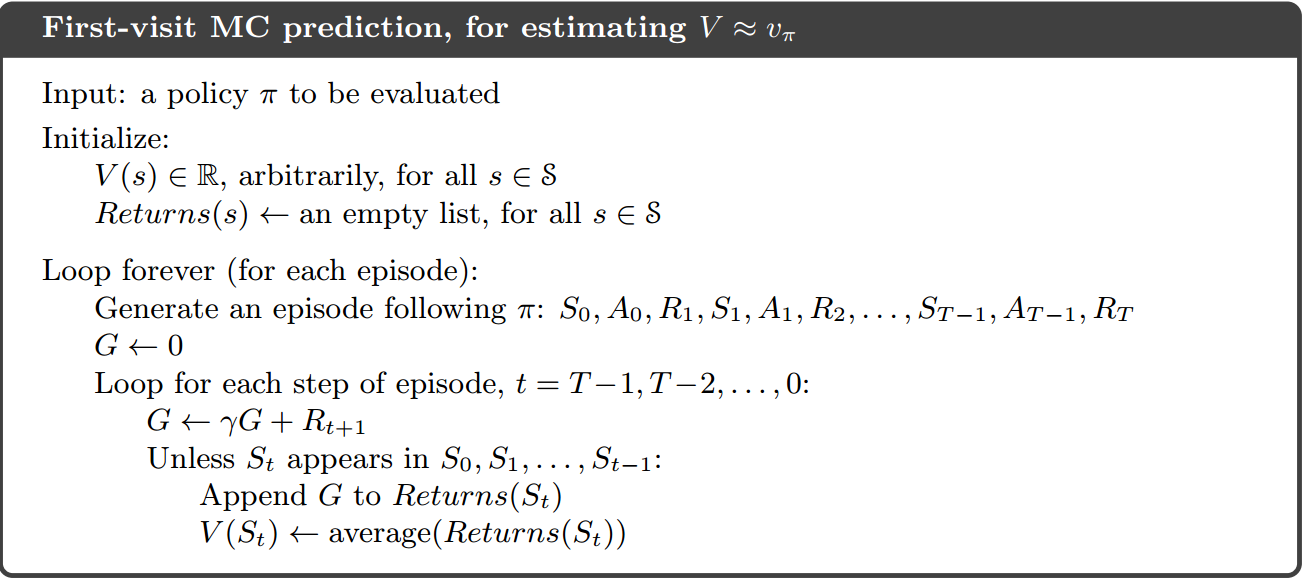
\includegraphics[scale = 0.3]{First_visit_MC_pred.png}}
\end{minipage}
\caption{\footnotesize{\textbf{First visit MC prediction}}}
\label{fig: First_visit_MC_pred}
\end{figure}

By the law of large numbers the sequence of averages of these estimates converges to their expected value. Each average is itself an unbiased estimate, and the standard deviation of its error falls as $1/\sqrt{n}$, where $n$ is the number of returns averaged. 



\section{Monte Carlo Methods for Control}
If a model is not available, then it is particularly useful to estimate \emph{action values} (the values of state-action pairs) rather than \emph{state values}. Without a model, the state-value is not sufficient since we cannot one simply looks ahead one step and chooses whichever action leads to the best combination of reward and next state.  One must explicitly estimate the value of each action in order for the values to be useful in suggesting a policy. Thus, one of our primary goals for Monte Carlo methods is to estimate $q_{*}$. Note that 
\begin{align*}
q_{\pi}(s, a) &= \E{\pi}{G_{t} | S_{t} = s, A_{t} = a} \\
&\approx \frac{1}{N(s, a)}\sum_{t}^{T(s,a)}G_{t}
\end{align*} where $N(s,a) = |T(s,a)|$, $T(s,a):=\set{t: S_{t} = s, A_{t} = a, t=0,..,T-1, ...}$ for every-visit MC or the timestamps for the first visit for all episodes. 

Conveniently, the same process as in previous section works for action values.  The Monte Carlo methods compute average returns starting in state $s$, taking actions $a$,  and thereafter following policy $\pi$. A state-action pair $s$, $a$ is said to be \emph{visited} in an episode if ever the state s is \emph{visited} and action $a$ is \emph{taken} in it. The \emph{every-visit MC method} estimates the value of a state-action pair as the average of the returns that have followed all the visits to it. The \emph{first-visit MC method} averages the returns following the first time in each episode that the state was visited and the action was selected. These methods converge quadratically, as before, to the true expected values as the number of visits to each state–action pair approaches infinity.

\begin{figure}
\begin{minipage}[t]{1\linewidth}
  \centering
  \centerline{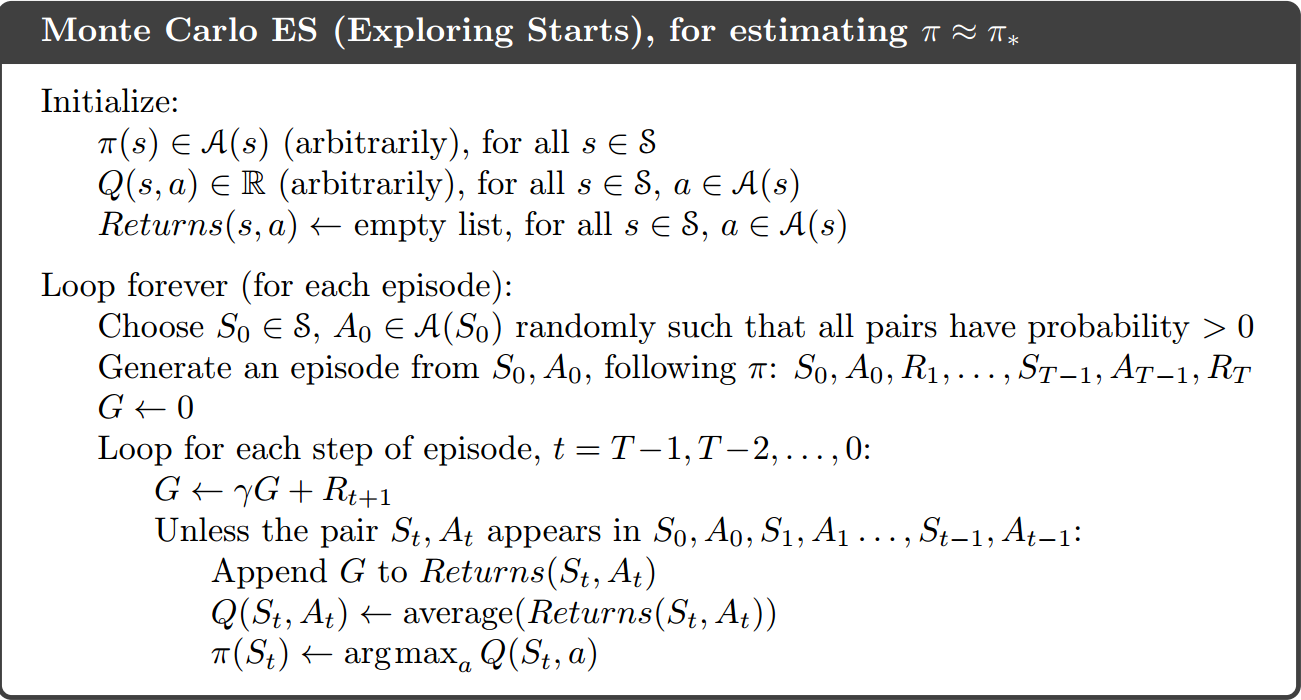
\includegraphics[scale = 0.3]{MC_ES.png}}
\end{minipage}
\caption{\footnotesize{\textbf{MC control with exploring starts}}}
\label{fig: MC_ES}
\end{figure}

The challenge for estimating action value via MC is that many state-action pairs may \emph{\textbf{never be visited}}, esp. for a deterministic policy $\pi$, when one will only observe returns only for one of actions from each state.  With no returns to average, the Monte Carlo estimates of the other actions will not improve with experience. To compare alternatives we need to estimate the value of \emph{\textbf{\underline{all}}} \emph{the actions from each state}, not just the one we currently favor. This is the \textbf{exploration-exploiation tradeoff}, as discussed in the multi-armed bandit. 

For \emph{policy evaluation} to work for action values, we must assure \emph{continual exploration}. One way to do this is by specifying that the episodes \emph{\textbf{start} in a state-action pair}, and that every pair has a nonzero probability of being selected as the start. This guarantees that \underline{all state-action pairs will be visited} an infinite number of times in the limit of an infinite number of episodes. We call this the assumption of \emph{\textbf{exploring starts}}. Figure \ref{fig: MC_ES} shows the algorithm for \textbf{Monte Carlo with exploring starts}. Note that at the initial step of the algorithm, a random state-action pair $(S_{0}, A_{0})$ is generated where no policy used for generating action. Then the policy $\pi$ is used to generate the episodes afterwards. 

The exploring start method is not very reliable esp. when learning directly from actual interaction with an environment. In that case the starting conditions are unlikely to be so helpful. The most common alternative approach to assuring that all state–action pairs are encountered is to consider only policies that are stochastic with a nonzero probability of selecting all actions in each state.


\subsection{Monte Carlo for Policy Iteration}
Given the estimation of action-value function $q$, we can choose the greedy policy $\pi(s) = \argmax_{a}q(s, a)$. \emph{Policy improvement} then can be done by constructing each $\pi_{k+1}$ as the greedy policy with respect to $q_k$. This greey policy $\pi_{k+1}$ is known to improve over existing policy $\pi_{k}$ by the \emph{policy improvement theorem}. From last section, we can use Monte Carlo Methods for policy evaluation. Then we have generalized policy iteration again
\begin{align*}
\pi_{0} \xrightarrow{E} q_{\pi_0} \xrightarrow{I} \pi_{1} \xrightarrow{E} q_{\pi_1}  \xrightarrow{I} \ldots \xrightarrow{I} \pi_{*} \xrightarrow{E} q_{*}
\end{align*} where $ \xrightarrow{E}$ denotes a policy evaluation and $\xrightarrow{I}$ denotes a policy improvement. Unlike DP in previous chapter, Monte Carlo methods can be used to find optimal policies given only sample episodes and no other knowledge of the environment’s dynamics. 

For Monte Carlo policy iteration it is natural to alternate between evaluation and improvement on an episode-by-episode basis. After \textbf{each episode}, the observed returns
are used for \emph{policy evaluation}, and then the policy is improved at \emph{\textbf{all the states visited in the episode}}.  In Monte Carlo ES, all the returns for \emph{each state-action pair} are accumulated and averaged, \underline{irrespective of what policy} was in force when they were observed. \textbf{Stability} is achieved only when both the policy and the value function are \textbf{optimal}. Convergence to this optimal fixed point seems inevitable as the changes to the action-value function decrease over time, but has not yet been formally proved.

The convergence guarantee for Monte Carlo Policy Iteration is based on two unlikely assumptions above. 
\begin{enumerate}
\item the episodes have \textbf{exploring starts}

\item policy evaluation could be done with an infinite number of episodes.
\end{enumerate} To obtain a practical algorithm we will have to remove both assumptions, which will be considered later. 

Removing the second assumption is relatively easy. In both DP and Monte Carlo cases there are two ways to solve the problem. One is to hold firm to the idea of approximating $q_{\pi_k}$ in each policy evaluation. Measurements and assumptions are made to obtain \emph{\textbf{bounds}} on the magnitude and \emph{probability of error} in the estimates, and then \underline{\emph{sufficient steps}} are taken during each policy evaluation to assure that these bounds are sufficiently small. This approach can probably be made completely satisfactory in the sense of guaranteeing correct convergence \emph{up to some level of approximation}. However, it is also likely to require far \textbf{too many episodes} to be useful in practice on any but the smallest problems.

The second approach is to give up trying to complete policy evaluation before returning to policy improvement. On each evaluation step we move the value function toward $q_{\pi_k}$, but we do not expect to actually get close except over many steps. One extreme form of the idea is value iteration, in which only one iteration of iterative policy evaluation is performed between each step of policy improvement.

\section{On-policy and Off-policy learning without exploring starts}
Without exploring starts, the only general way to ensure that \underline{all actions are selected infinitely often} is for the agent to continue to select them. There are two approaches to ensuring \textbf{continual exploration}:
\begin{itemize}
\item \textbf{\emph{On-policy} methods}. On-policy methods attempt to evaluate or improve the \emph{policy} that is used to \underline{make decisions}.

\item \textbf{\emph{Off-policy} methods}. Off-policy methods evaluate or improve a policy \textbf{different} from that used to \underline{generate the data}. In this case we say that learning is from data "off" the target policy. There are 
\begin{itemize}
\item \textbf{target policy}, i.e.  the policy being learned about, denoted as $\pi(a|s)$; 
\item \textbf{behavior policy}, i.e. the policy used to generate behavior, denoted as $b(a|s)$
\end{itemize}  
\end{itemize}

\begin{figure}
\begin{minipage}[t]{1\linewidth}
  \centering
  \centerline{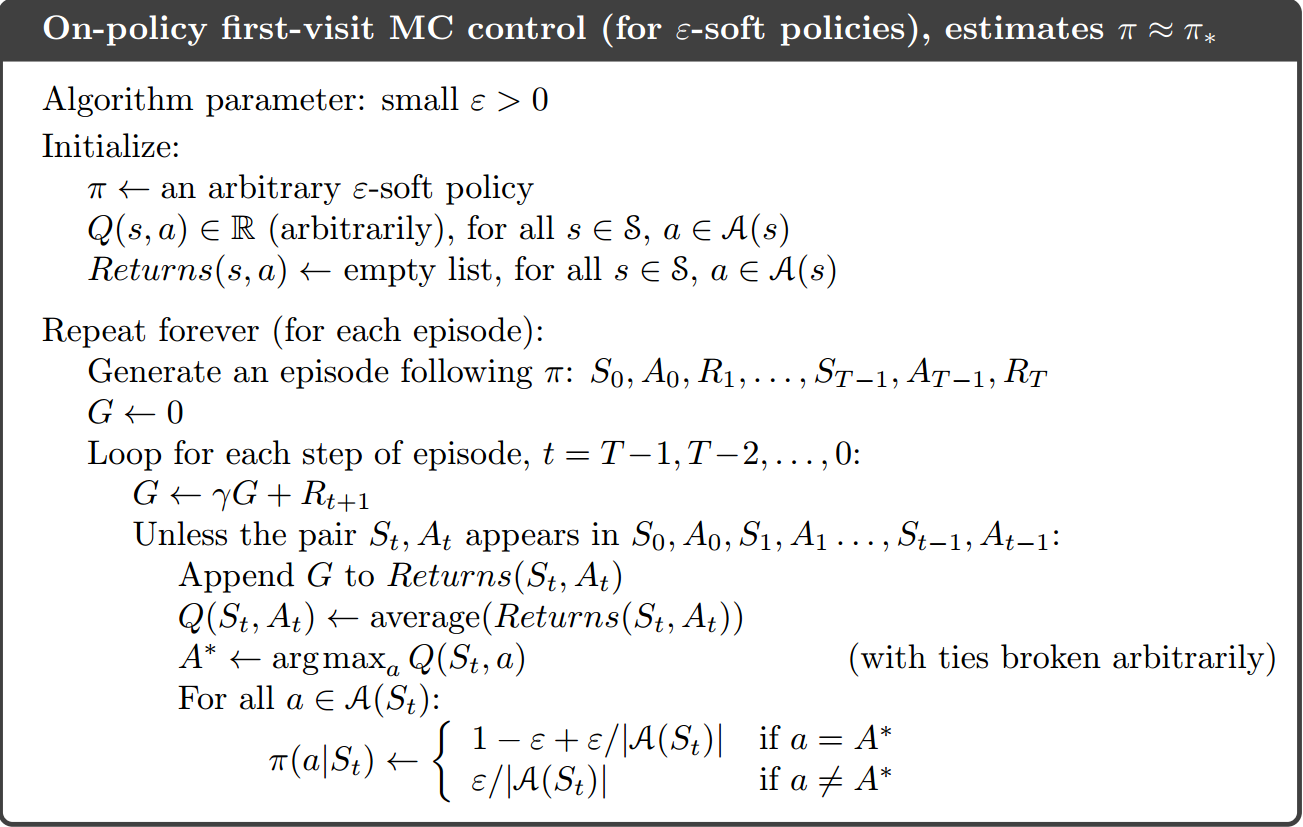
\includegraphics[scale = 0.3]{on_policy_mc_eps_soft.png}}
\end{minipage}
\caption{\footnotesize{\textbf{On-policy Monte Carlo with epsilon-soft policies}}}
\label{fig: on_policy_mc_eps_soft}
\end{figure}

\subsection{On-policy method with $\epsilon$-soft policies}
In on-policy control methods the policy is generally \emph{\textbf{soft}}, meaning that  $\pi(a|s) > 0$ for all $s \in \cS$ and all $a \in \cA(s)$, but gradually shifted closer and closer to a deterministic optimal policy. For example, the \emph{$\epsilon$-greedy} algorithms discussed in Multi-armed Bandit algorithm  are examples of \emph{\textbf{$\epsilon$-soft}} policies, defined as policies for which $\pi(a|s) \ge \frac{\epsilon}{|\cA(s)|}$ for all states and actions, for some $\epsilon \ge 0$. This ensures that all states are visited infinitely in the long run. 

Note that the overall idea of on-policy Monte Carlo control is still that of \emph{GPI}. In this case, using the learned greedy policy via policy improvement would prevent further exploration of nongreedy actions.  On the other hand, as long as the new policy moves \emph{towards greedy policy}, we would see GPI continue towards optimal solution.  For any $\epsilon$-soft policy, $\pi$, any $\epsilon$-greedy policy with respect to $q_{\pi}$ is guaranteed to be \textbf{better} than or equal to $\pi$. Figure \ref{fig: on_policy_mc_eps_soft} describes the on-policy first-visit Monte Carlo control for $\epsilon$-soft policy. Here the policy select optimal action $\argmax_{a}q(s,a)$ with probability $1-\epsilon+\frac{\epsilon}{|\cA(s)|}$ and other uniformly randomly with probability $\frac{\epsilon}{|\cA(s)|}$.

Note that by nature, this algorithm will \underline{not converge to optimal policy} $\pi_{*}$, which is a deterministic greedy policy. Instead it will \textbf{converge to an $\epsilon$-greedy policy} that is close enough to the optimal policy with random action selection. This is because any $\epsilon$-greedy policy $\pi'$ with respect to $q_{\pi}$ is an improvement over any $\epsilon$-soft policy $\pi$ by the policy improvement theorem.  
\begin{align*}
q_{\pi}(s, \pi'(s)) &= \sum_{a}\pi'(a|s) q_{\pi}(s, a) \\
&= \frac{\epsilon}{|\cA(s)|}\sum_{a}q_{\pi}(s, a) + (1-\epsilon)\max_{a\in \cA(s)}q_{\pi}(s, a) \\
&\text{since }\max_{a\in \cA(s)}q_{\pi}(s, a) \ge \sum_{a}w_a\,q_{\pi}(s, a) \\
&\ge  \frac{\epsilon}{|\cA(s)|}\sum_{a}q_{\pi}(s, a) + (1-\epsilon)\sum_{a}\frac{\pi(s|a) -  \frac{\epsilon}{|\cA(s)|}}{1-\epsilon}q_{\pi}(s, a) \\
&=  \sum_{a}\pi(s|a)q_{\pi}(s, a) \\
&= v_{\pi}(s)
\end{align*} Thus $v_{\pi'} \ge v_{\pi}$ for all $s$, $\pi' \ge \pi$. This \emph{suboptimal} solution is a \textbf{compromise} for on-policy learning for the exploration-exploitation tradeoff.

$\epsilon$-soft policy describes an environment where with probability $1-\epsilon$ it behaves like the old environment and with probability $\epsilon$ it choose a new, uniformly random action. The best one can do in this new environment with general policies is the same as the best one could do in the original environment with $\epsilon$-soft polices. The optimal state-value  functions for $\epsilon$-soft polices are like
\begin{align*}
\tilde{v}_{*}(s) &=  \frac{\epsilon}{|\cA(s)|}\sum_{a}\tilde{q}_{*}(s, a) + (1-\epsilon)\max_{a\in \cA(s)}\tilde{q}_{*}(s, a) \\
&=\frac{\epsilon}{|\cA(s)|}\sum_{a}\sum_{s'}\sum_{r}p(s', r|s, a)\brac{r + \gamma \tilde{v}_{*}(s')}+ (1-\epsilon)\max_{a\in \cA(s)}\sum_{s'}\sum_{r}p(s', r|s, a)\brac{r + \gamma \tilde{v}_{*}(s')}
\end{align*} This makes sure that the Generalized Policy Iterations works for  $\epsilon$-soft polices.

\subsection{Off-policy prediction with importance sampling}
The exploration-exploitation tradeoff states that all algorithms need to learn action values conditional on subsequent \underline{\emph{optimal}} behavior, but they need to behave non-optimally in order to \underline{\emph{explore}} all actions (to \emph{find} the optimal actions), i.e. learning optimal behavior while maintaining \emph{continual exploration}. 

\begin{itemize}
\item On-policy methods are generally simpler and are considered first. Off-policy methods require additional concepts and notation, and because the data is due to a different policy, off-policy methods are often of greater variance and are slower to converge.

\item Off-policy methods also have a variety of additional uses in applications. For example, they can often be applied to learn from data generated by a conventional non-learning controller, or from a human expert. Off-policy learning is also seen by some as key to learning multi-step predictive models of the world’s dynamics. 

\item On-policy methods have to make a sacrifice to the performance by choosing sub-optimal policy in order to keep exploring. Off-policy methods do not have this issue. 
\end{itemize}

In this section, assume both target and behavior policy are fixed and given. We are considering the off-policy prediction problem, i.e. estimating $v_{\pi}$ and $q_{\pi}$, where episodes follow policy $b\neq \pi$. Also we made the \emph{assumption of \textbf{coverage}}: i.e. $\text{supp}(\pi(\cdot|s))  \subseteq \text{supp}(b(\cdot|s))$. That means that every action taken under $\pi$ is also taken, at least occasionally, under $b$; or, for action $a$, $\pi(a|s) > 0$ implies $b(a|s) >0$. The behavior policy $b$ has to be \emph{stochastic} to provide coverage while the target policy $\pi$ could be \emph{deterministic}. 



Almost all off-policy methods utilize \textbf{importance sampling}, a general technique for estimating expected values under one distribution given samples from another. We apply importance sampling to off-policy learning by weighting returns according to the relative probability of their trajectories occurring under the target and behavior policies, called \emph{\textbf{the importance-sampling ratio}}.
\begin{align*}
P(A_{t}, S_{t+1}, A_{t+1}, \ldots, S_{T} \big| S_{t}, A_{t:T-1} \sim \pi ) &= \prod_{k=t}^{T-1}\pi(A_{k}|S_{k})p(S_{k+1} | S_{k}, A_{k})
\end{align*} where $p$ is the state-transition probability. The importance-sampling ratio is defined as
\begin{align}
\rho_{t:T-1} &= \frac{P(A_{t}, S_{t+1}, A_{t+1}, \ldots, S_{T} \big| S_{t}, A_{t:T-1} \sim \pi )}{P(A_{t}, S_{t+1}, A_{t+1}, \ldots, S_{T} \big| S_{t}, A_{t:T-1} \sim b )}  \nonumber\\
&= \frac{\prod_{k=t}^{T-1}\pi(A_{k}|S_{k})p(S_{k+1} | S_{k}, A_{k})}{ \prod_{k=t}^{T-1}b(A_{k}|S_{k})p(S_{k+1} | S_{k}, A_{k})} \nonumber\\
&= \prod_{k=t}^{T-1}\frac{\pi(A_{k}|S_{k})}{b(A_{k}|S_{k})} \label{eqn: importance_sample_ratio}
\end{align} The importance sampling ratio ends up depending only on the two policies and the sequence, not on the MDP.

\begin{figure}
\begin{minipage}[t]{1\linewidth}
  \centering
  \centerline{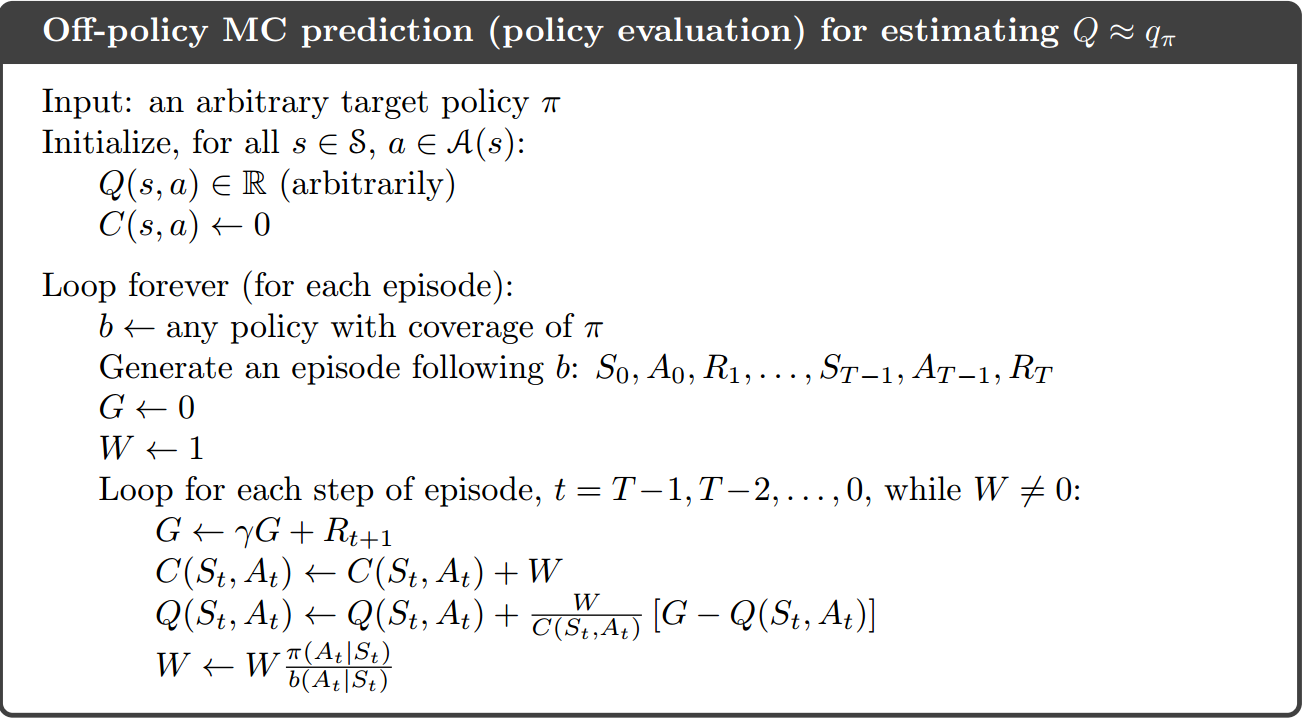
\includegraphics[scale = 0.3]{off_policy_mc_prediction.png}}
\end{minipage}
\caption{\footnotesize{\textbf{Off-policy every-visit Monte Carlo prediction with weighted importance sampling}}}
\label{fig: off_policy_mc_prediction}
\end{figure}

With importance sampling, the estimate of state-value function $v_{\pi}(s)$ can be obtained by average returns based on policy $b$ and ratio $\rho$
\begin{align}
v_{\pi}(s)&= \E{b}{\rho_{t:T-1}G_{t} | S_{t}=s}  \nonumber\\
&\approx \frac{1}{|N(s)|}\sum_{t \in N(s)}\rho_{t:T(t)-1}G_{t} \label{eqn: MC_IS}
\end{align} where $N(s) := \set{t: S_{t} = s}$ for an every-visit method; for a first-visit method, $N(s)$ would only include time steps that were first visits to $s$ within their episodes. And let $T(t)$ be the first time of termination following time $t$ (i.e. end of current episode), and $G_t$ denote the return after $t$ up through $T(t)$. The above method is called \emph{\textbf{ordinary importance sampling}}.

An important alternative is \emph{\textbf{weighted importance sampling}}, which uses a weighted average, defined as
\begin{align}
V(s) &:= \frac{\sum_{t \in N(s)}\rho_{t:T(t)-1}G_{t}}{\sum_{t \in N(s)}\rho_{t:T(t)-1}}, \label{eqn: MC_weighted_IS}
\end{align} or zero if the denominator is zero. 

Formally, the difference between the first-visit methods of the two kinds of importance sampling is expressed in their \underline{biases and variances}. \emph{Ordinary importance sampling} is  \underline{\emph{\textbf{unbiased}}} whereas \emph{weighted importance sampling} is \underline{\emph{biased}} (though the bias converges asymptotically to zero). On the other hand, the variance of ordinary importance sampling is in general \underline{\emph{\textbf{unbounded}}} because the variance of the ratios can be unbounded, whereas in the weighted estimator the largest weight on any single return is  \underline{\textbf{\emph{one}}}. In fact, assuming bounded returns, the variance of the weighted importance-sampling estimator \underline{converges to zero} even if the variance of the ratios themselves is infinite. In practice, the weighted estimator usually has dramatically lower variance and is strongly preferred.  The every-visit methods for ordinary and weighed importance sampling are \underline{both biased}, though, again, the bias falls asymptotically to zero as the number of samples increases.

\subsection{incremental update of off-policy prediction}
In ordinary importance sampling, the returns are scaled by the importance sampling ratio $\rho_{t:T(t)-1}$, then simply averaged. For these methods we can again
use the incremental methods introduced in Multi-armed Bandit, but using the scaled returns in place of the rewards of that chapter. 

In weighted importance sampling, suppose we have a sequence of returns $G_1, G_2, . . . , G_{n-1}$, all starting in the same stateand each with a corresponding random weight $W_i$ (e.g., $W_i = \rho_{t:T(t_{i})-1}$). We wish to form the estimate
\begin{align*}
V_{n} &:=  \frac{\sum_{k=1}^{n-1}W_{k}G_{k}}{\sum_{k=1}^{n-1}W_{k}}, \quad n\ge 2
\end{align*} We can derive an incremental update as below:
\begin{align}
V_{n+1} &= V_{n} + \frac{W_{n}}{C_{n}}\brac{G_{n} - V_{n}}, \quad n\ge 1 \label{eqn: incremental_update_weighted_IS} \\
     C_{n+1} &= C_{n} + W_{n+1} \label{eqn: incremental_update_weighted_IS2}
\end{align} where $C_{0}=0$. The Figure \ref{fig: off_policy_mc_prediction} contains a complete episode-by-episode incremental algorithm for Monte Carlo policy evaluation. The algorithm is nominally for the off-policy case, using weighted importance sampling, but applies as well to the on-policy case just by choosing the target and behavior policies as the same.

\section{Off-policy Monte Carlo Control}
\begin{figure}
\begin{minipage}[t]{1\linewidth}
  \centering
  \centerline{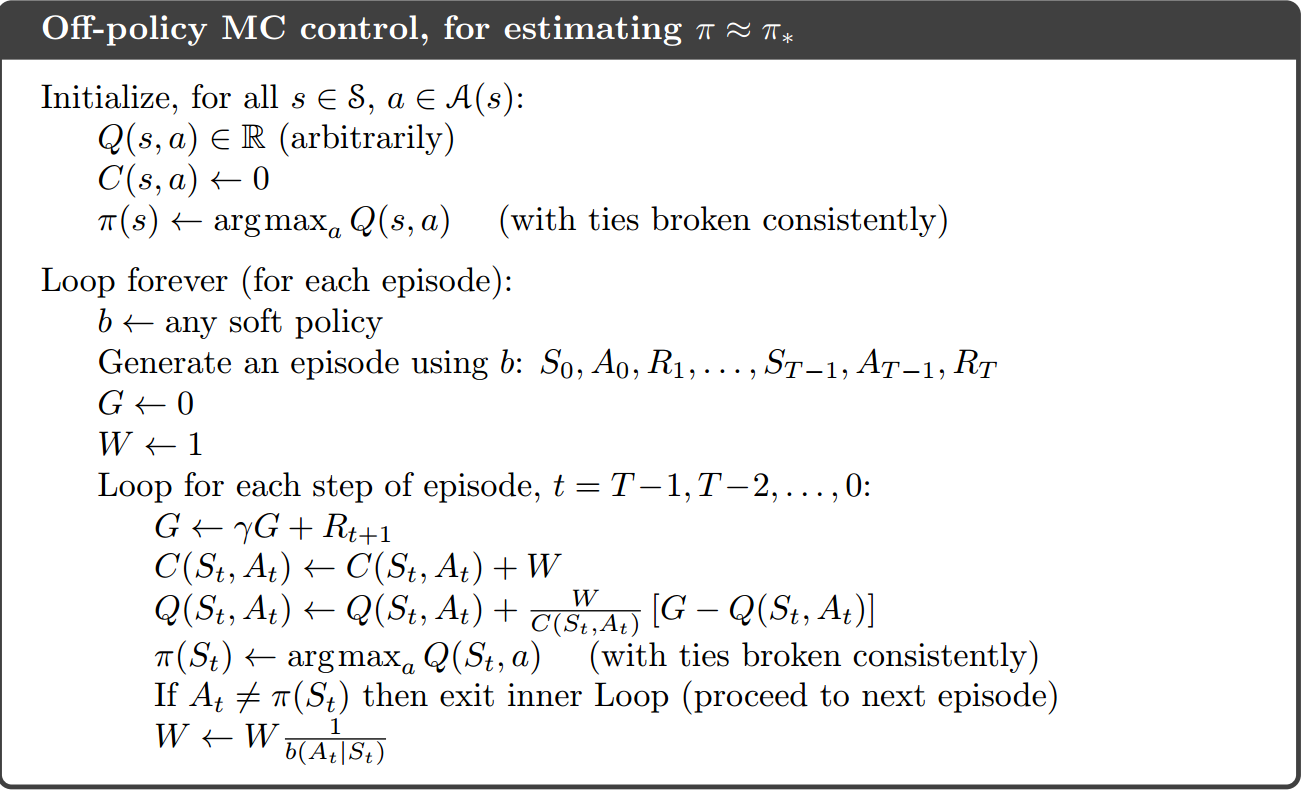
\includegraphics[scale = 0.3]{off_policy_mc_control.png}}
\end{minipage}
\caption{\footnotesize{\textbf{Off-policy Monte Carlo Control}}}
\label{fig: off_policy_mc_control}
\end{figure}

Combine two sections above, we obtain the \textbf{off-policy control algorithm}. Recall that the distinguishing feature of on-policy methods is that they \emph{estimate the value} of a policy while \underline{using it for control}. In off-policy methods these two functions are separated. An advantage of this separation is that the target policy may be \emph{deterministic} (e.g., greedy), while the behavior policy can \emph{continue to sample} all possible actions. They follow the behavior policy while learning about and
improving the target policy. To maintain continual exploration, the behavior policy is required to be \emph{soft}. 

Figure \ref{fig: off_policy_mc_control} shows the off-policy Monte Carlo Control using weighted importance sampling. This follows the GPI to estimate $\pi_{*}$ and $q_{*}$. The target policy $\pi \approx \pi_{*}$ is the greedy policy with respect to $Q$, which is an estimate of $q_{\pi}$. The behavior policy need to provide coverage for target $\pi$. Thus choosing the $\epsilon$-soft policy.

A potential problem is that this method learns only from the \emph{tails of episodes}, when all of the remaining actions in the episode are \emph{greedy}. If nongreedy actions are common, then learning will be \textbf{slow}, particularly for states appearing in the early portions of long episodes. Potentially, this could greatly slow learning. There has been insufficient experience with off-policy Monte Carlo methods to assess how serious this problem is. 

\newpage
\bibliographystyle{plainnat}
\bibliography{reference.bib}
\end{document}